In the previous chapters, we analyzed two core parts of our EasyFly programming environment: the Communication and the Coordination frameworks.
At this point, these two frameworks can appear isolated and useless for reaching our final objective of creating a simple programming environment for drone applications in HDI research.

To leverage the real potentiality of these two frameworks, we need a principal actor that links all the pieces together and transforms our EasyFly from being a software library to a complete programming environment for drone applications.

Here is where the Extended Crazyflie (ECF) comes into play: the simplest but most effective component of EasyFly. 
This component is a centralized unit that wraps and links together all the functionalities of our programming environment. 
Moreover, it directly connects to a Crazyflie 2.1 and is used as a unique interface to interact with and control the drone's behavior.

In this chapter, we will present the Extended Crazyflie component, analyzing in detail its structure and the main functionalities. 
We will conclude by presenting a possible solution for the use case scenario described in the previous chapter (see Secion\ref{subsec:coordination_manager}),
by using this approach.


\section{The Structure and Design Principles of Exteded Crazyflie}\label{sec:ecf_structure_design}

Learning a new programming environment for drone applications can be really challenging. 
Usually, when used for the first time, the setup phase of a programming environment is very complicated and full of issues. 

Since EasyFly is intended to be a simple and accessible programming environment for drone applications, the learning curve must be as fast as possible.
For this reason, we have been focused on two main objectives:
\begin{itemize}
    \item Automation of all processes that are usually performed in most drone applications
    \item Centralization to a single component for all the functionalities provided inside the programming environment
\end{itemize}

In particular, the first objective should allow a beginner developer to set up the environment quickly and be ready to develop in a few minutes. 
By simply knowing the address of the Crazyflie 2.1, the developer should be able to connect and control it without any effort.

The second objective should allow a beginner developer to know all the functionalities they can use to control the drone by simply looking at the API of one single component. 
Whatever is accessible from that component is all they need to control the Crazyflie in the desired manner.

The ECF component structure is simple and follows the facade design pattern:
The Facade pattern is a design pattern in software engineering that provides a simplified interface to a complex system of classes, interfaces, and objects. 
It is commonly used to hide the complexity of a system; it presents a simple and unified interface and perfectly fits our needs.

To effectively implement the facade pattern, the ECF component initializes and keeps the references of the other components of the programming environment, 
such that any part of the EasyFly is accessible via the ECF component.

As shown in Figure~\ref{fig:ecf_structure}, the ECF component is composed of three parts:
\begin{itemize}
    \item The Communication Framework
    \item The Coordination Framework
    \item A set of additional modules
\end{itemize}

The frameworks discussed in the previous chapters represent the first two sections of the structure. 
In particular, we included one instance for each framework's manager in the ECF component.
We have one Logging and one Parameters Manager for the Communication Framework, while for the Coordination Framework, we have one Coordination Manager.

The last section of the structure is represented by a set of Modules, each of which is in charge of introducing additional functionalities to the environment. 
The type of modules instantiated is automatically determined by the ECF component and depends on the current configuration mounted onboard the Craziflie 2.1 (see Section~\ref{subsec:ecf_modules_overview}).
We will enter more in detail about such modules in the following sections; for now, let us consider these modules as an encapsulated set of functionalities.
 
\sidecaptionvpos{figure}{c}
\begin{SCfigure}[\sidecaptionrelwidth][h]
    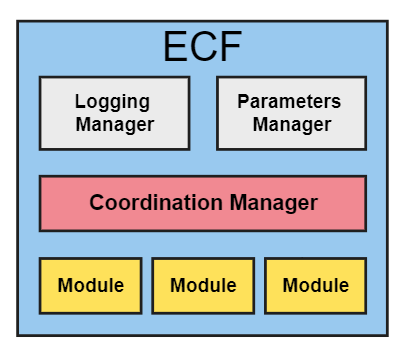
\includegraphics[width=0.5\textwidth]{ecf/ecf_structure}
    \caption{Extended Craziflie component structure}\label{fig:ecf_structure}
\end{SCfigure}

The successful implementation of the facade design pattern allows for a centralized interface, accomplishing the second objective previously stated.
Still, the Extended Crazyflie does not include any automation processes, allowing users to eliminate the expensive setup phase and lowering the learning curve.

To understand how the ECF accomplishes this other objective, we need to take it a step further and analyze better how the structure described above is created when a new instance of the ECF is created.
In Figure~\ref{fig:ecf_sequence}, we can see the sequence of the operations performed at the component's initialization.
As we anticipated, the ECF is directly linked to a Crazyflie 2.1, so before getting an instance of the main component, we need to know the address (uri) of the Crazyflie that we desire to connect.

The first thing the component does is initialize the communication protocol drivers from the ground station to the drone and instantiate the connection between the two.
After that connection is established, the ECF creates a unique instance for the Parameter Manager, the Logging Manager, and the Coordination Manager and stores them in its local storage.

To initialize the software sensing used for estimating its state (see Section~\ref{sec:state_estimate_and_control}) with a clean initial state, resetting the estimators before taking off is usually helpful. 
Indeed, by default, the ECF uses the Parameters Manager to reset the state estimate right after the creation of the Managers.

The last operation in the initialization phase is the creation of the additional modules. 
Since the modules creation process is automatic and depends on the current configuration of decks onboard, the ECF needs to know the current configuration.
To do so, it uses the Parameters Managers; by reading some parameters, it can easily determine which decks are mounted onboard.

Each module can be viewed as a simple component, so for each module needed, the ECF creates a new instance of the module's component and stores it in its local storage. 
The ECF stores its modules in a local repository so that each module's instance can be retrieved straightforwardly by knowing the module's type.

\begin{figure}[h]
    \centering
    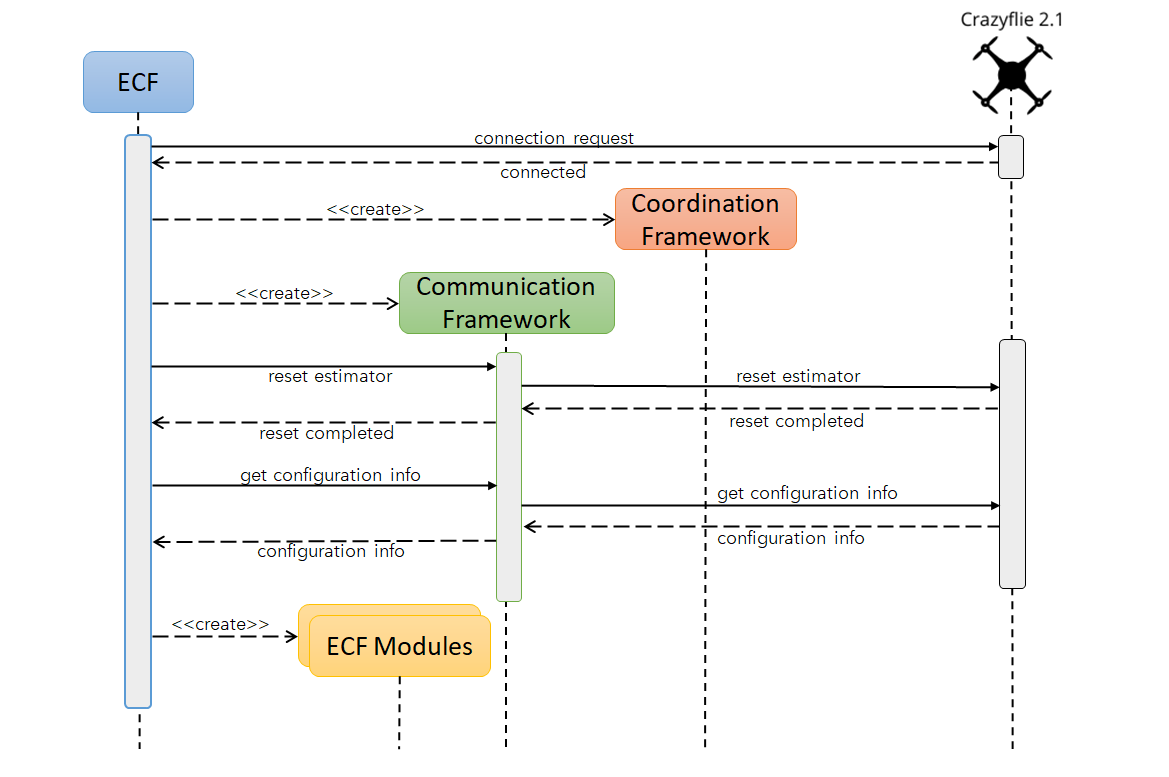
\includegraphics[width=0.9\textwidth]{ecf/ecf_sequence} 
    \caption[ECF initialization sequence diagram]{The sequence diagram of the initialization of the Extended Craziflie shows the operations performed to have a working instance of the component}\label{fig:ecf_sequence}
\end{figure}


\subsection{Extended Crazyflie Modules}\label{subsec:ecf_modules_overview}
As we have seen, the Extended Crazyflie component instantiates a set of modules, each of which can be viewed as a container of functionalities.
So far, it is still unclear what such modules are, what their structure is, what those added functionalities are, and last but not least, which type of modules the EasyFly programming environments have. 

In this section, we will deeply understand ECF Modules, and we will answer all of these questions.
Before entering into the details of modules, let's step back and understand the origin of the idea behind those modules.
To make this, think back to the use case scenario solved in Section~\ref{subsec:coordination_manager}, and more generally, think of the process we proposed to develop a drone application easily using EasyFly.

The steps that we followed were:
\begin{itemize}
    \item Define the state of the application
    \item Setup the Coordination Framework to handle that state
    \item Setup the Logging Manager to update correctly that state
    \item Define how and when reacting to state changes
\end{itemize}

Apart from the first step, which is usually the most complex and depends mostly on the application scenario, we can say that the other steps are made of identical operations, almost independently from the application.
Apparently, the first step, which defines the state, is indeed profoundly diverse across different applications.
But if we analyze the possible states that the application can use, we can notice that the state is usually composed only of internal and sensed data; 
resulting in a very limited set of variables.
Ultimately, we will use the same state or a union of “standard” parts for most of the applications. 

For example, the estimated position information is always crucial in almost any drone application. 
Hence, we could define a component that automatically creates a state inside the Coordination Manager and keep it updated.

An ECF Module is a component that defines a \textit{standard state}.
Using the Communication and Coordination frameworks, it updates this state and makes it available through a \textit{standard Observable} inside the Coordination framework.

By using standard modules, we reduced and focused (for most of the application) the development process to a single task: defining how and when reacting to state changes.
The structure of an ECF module is shown in Figure~\ref{fig:ecf_module_structure}: it has a list of state variables, each of which is continuously updated every time a new value is available. 
So, at any point, these variables contain the last value known read from the Crazyflie for that variable.

As the last fundamental component, the ECF Module can include some utility functions strictly related to the state they define. 
In the next chapter (see Chapter~\ref{ch:modules}), we will better analyze ECF modules and their utility functions.

\sidecaptionvpos{figure}{c}
\begin{SCfigure}[\sidecaptionrelwidth][h]
    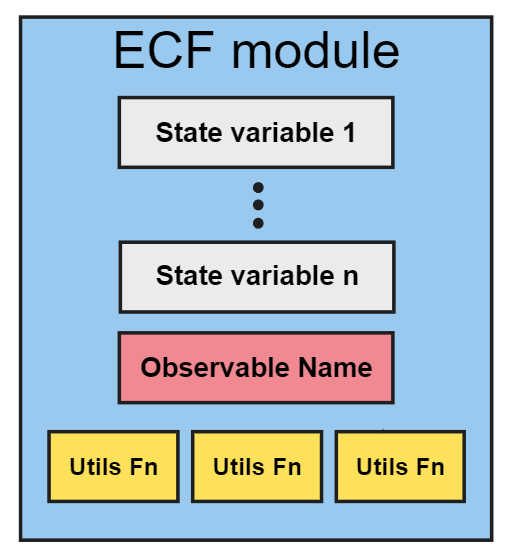
\includegraphics[width=0.5\textwidth]{ecf/ecf_module}
    \caption{Extended Craziflie Module internal structure}\label{fig:ecf_module_structure}
\end{SCfigure}

To answer the last question: what type of ECF Modules exist in EasyFly? 
We need to consider valuable states to become \textit{standard states}.

Since our state can be defined either by internal state or by external sensed data, we decided to create the following Modules:
\begin{itemize}
    \item Internal State
    \begin{itemize}
        \item State Estimate Module
        \item Battery Module
    \end{itemize}
    
    \item Sensed Data State
    \begin{itemize}
        \item Multiranger Module
        \item Z Ranger Module
        \item Flow Deck Module
        \item Lighthouse Module
        \item Ai Deck Module
    \end{itemize}
\end{itemize}


\subsection{Use Case Scenario's Solution}\label{subsec:solution_use_case_scenario}

We analyzed in detail what ECF is and what its structure is. 
Moreover, we described the purpose and the functioning of its core part, the ECF Modules. 

At this point, we will show a possible solution to the same use case scenario we solved in Chapter~\ref{subsec:coordination_manager}, this time using the functionalities of the ECF component.
We purposely selected the same example that is already solved to see how much complexity the ECF handles, hiding it from the developer.

For simplicity, we rewrite the specification of the example:
\begin{displayquote}
    For the drone application that we are developing, we need the drone to be maintained not too close to the walls of the flight area. 
    Specifically, it must maintain a safe distance of 0,5 meters from the walls.
\end{displayquote}

If we analyze the requirements, we can say that the only information we need to know to control the drone is the distance from the wall. 
For that purpose, we can use the Multiranger deck, which will give us the distance from the nearest obstacle in the four directions (see Section~\ref{deck:multi_ranger}).
Before going straight forward to the implementation, we should briefly introduce the module that we will use in this example: the Multiranger module.
The Multiranger module is an ECF module which defines a Sensed Data State as follows:
 
\begin{lstlisting}[language=Python]
    State = {
        "left": "Distance from nearest obstacle on the left",
        "right": "Distance from nearest obstacle on the right",
        "front": "Distance from nearest obstacle on the front",
        "back": "Distance from nearest obstacle on the back",
        "up": "Distance from nearest obstacle above"
    }
\end{lstlisting}

For this state, the Multiranger Module will create and keep updated an observable in the Coordination Manager. 
We can take advantage of this Observable and subscribe to it to react when the distance goes below 0.5 meters.
Here is the code of the example:

\begin{lstlisting}[language=Python]
from cflib.positioning.motion_commander import MotionCommander
from extension.decks.deck import DeckType
from extension.extended_crazyflie import ExtendedCrazyFlie

def safe_distance(multiranger_state : dict, mc : MotionCommander):
    if multiranger_state['left'] < 0.5:
        mc.right(0.5 - multiranger_state['left'])
    if multiranger_state['right'] < 0.5:
        mc.left(0.5 - multiranger_state['right'])
    if multiranger_state['front'] < 0.5:
        mc.back(0.5 - multiranger_state['front'])
    if multiranger_state['back'] < 0.5:
        mc.forward(0.5 - multiranger_state['back'])
    
with ExtendedCrazyFlie('radio://0/80/2M/E7E7E7E7E7') as ecf:
    with MotionCommander(ecf.cf) as mc:
        ecf.coordination_manager.observe(
        	observable_name= ecf.decks[DeckType.bcMultiranger]
                                .observable_name,
        	action= safe_distance,
            context= [mc],
        )
\end{lstlisting}

The code is organized into two main parts; the first part (\textit{lines 6-14}) is a function that contains the core logic of the application. 
If we analyze the signature, the function is an Action of the Coordination Framework: it takes as input the state of one observable and a MotionCommander object (the context) that is used to act on the Crazyflie effectively.

Four \textit{if} statements in the function's body check whether the distance from the nearest obstacle in one direction is below 0.5 meters. 
If that is the case, the function will use the Motion Commander object to move the drone in the opposite direction, bringing the drone back to a safe distance from the obstacle.

The second part (\textit{lines 17-23}) instead represents the only setup needed to create a working application. 
It comprises 2 \textit{with} statements and a single function call. 

Line 17 will create a new instance of Extended CrazyFlie and assign it to the variable \textit{ecf}.
As we know, all the setup operations are performed by creating the ECF component. 
Since we are mounting a Multiranger deck, it will also automatically create an instance of the Multiranger Module. 
The user with a single line of code is ready to use all its functionalities. 

Line 18 will create and initialize an instance of the Motion Commander. 
The Motion Commander is a functionality offered by the base cflib (see Section~\ref{sec:flight_control}), which exposes some functionalities that allow controlling the drone flight. 

In line 19, there is a call to the Coordination Manager to set up a subscription to the multiranger observable. 
In particular, we specified an action, the \textit{safe\_distance} function, and a context, the Motion Commander's instance \textit{mc}. 
In this way, every time the Multiranger Module updates the state, the \textit{safe\_distance} function will be called with the new state and the instance of the Motion Commander; if the function finds anomalies in the distance, it will apply a correction.

As we can see, the resulting code is clean and easy to understand, and all the complicated setup operations are handled automatically under the hood.
The Extended CrazyFlie component is a tool with much potential that allows the developer to start with the proper setup by writing a single line of code. 
Moreover, with standard ECF Modules, the developer can focus on the application's core business logic and reduce the skills needed to program an application and the time necessary to complete it effectively. 